\documentclass[a4paper]{article}

\usepackage{graphicx}
\usepackage{amsmath,amssymb}
\usepackage{minted}
\usepackage{multirow}
\usepackage{float}
\usepackage{algorithm}
\usepackage{algpseudocode}
\usepackage{todonotes}
\usepackage{forest}
\usepackage{xstring}
\usepackage{xcolor}
\usepackage[most]{tcolorbox}
\usepackage{xparse}
\usepackage{natbib}

\usetikzlibrary{graphs,graphdrawing}
\usegdlibrary{layered}

% for external graphviz
\input{/home/donkarlo/Dropbox/repo/nd_language_ai_project/src/nd_language_ai/formal/computer/programming/tex/latex/code_clips/external_graphviz.tex}

% for tags
\input{/home/donkarlo/Dropbox/repo/nd_language_ai_project/src/nd_language_ai/formal/computer/programming/tex/latex/part/control_sequence/kind/semtag/semtag.tex}

% for links
\input{/home/donkarlo/Dropbox/repo/nd_language_ai_project/src/nd_language_ai/formal/computer/programming/tex/latex/code_clips/seehere.tex}

\title{}
\date{}
\author{Mohammad Rahmani}

\begin{document}
   \maketitle
   \section{Self definition}
\seeherefooter{/nd_robotic_ai_learning_project/src/robot/part/mind/cognition/part/meta_cognition/part/self_conciousness/self_awareness/self/self.tex}

   \section{The dfiference between self and others}
      \seeherefooter{/nd_robotic_ai_learning_project/src/robot/part/mind/cognition/part/meta_cognition/part/self_conciousness/self_awareness/self/morkov_blanket/markov_blanket.tex}
      
      The self is grounded in self-referential processing, through which the brain distinguishes stimuli related to one's own person from non-self-related stimuli. From the neurological perspective , the self is recognized through self-referential processing, particularly involving cortical midline structures. \cite{northoff-2006-self-referential-processing-in-our-brain-a-meta-analysis-of-imaging-studies-on-the-self}.
      
      \cite{demekas-2020-an-investigation-of-the-free-energy-principle-for-emotion-recognition} uses Markov blankets to formalize the statistical boundary separating internal states of a system from external states, providing a basis for distinguishing self from other.
      It applies this framework within active inference to explain how an agent can infer both its own states and the states or intentions of other agents. This idea is used in \cite{friston-2013-life-as-we-know-it}
      to distinguish between self and other. 
      
      This ersearch also uses a probabilistic approach to make a distinction between self and other by recognizing the words written form other robot on shared balck board with high anomalies. 
      
   \section{What should be shared betwen robots}

      \begin{itemize}
         \item Variational auto encoder
      \end{itemize}

   \section{Examplary learned language}
      In the experiments section we will see an exmplary excepted langugae would contain words such as ``keep disatnce`` or ``move closer``
      \subsection{Sharing}
         \begin{figure}[H]
            \centering
            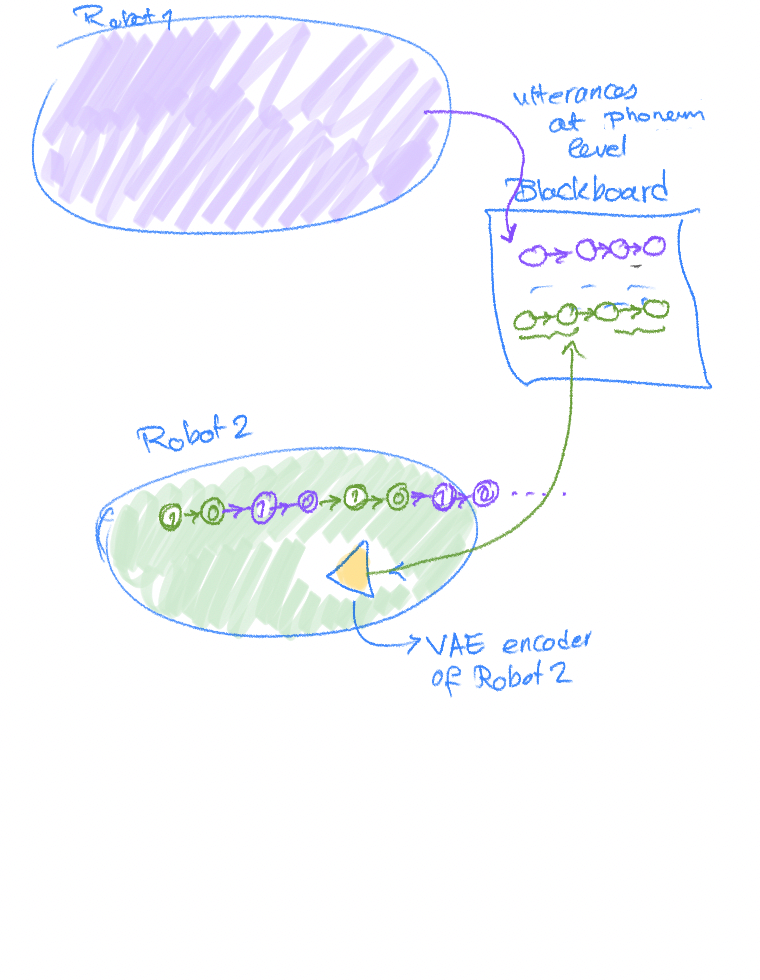
\includegraphics[width=0.9\textwidth]{mrs_communication.png}
            \caption{MRS mutual language building}
         \end{figure}

      \subsection{Blackboard}
         As in natural language, it is not possible to share the sensory data points. So on teh blackboard only sequences of phonems with a predefined sliding window length can be writetn.

   \section{Language}
      Jargon
      \begin{itemize}
         \item fly in prallel
         \item follow in narrow corridor
         \item wait until the other gets in parallel
      \end{itemize}



      \bibliographystyle{plainnat}
      \bibliography{/home/donkarlo/Dropbox/repo/nd_shared_research/bibliography/bibliography.bib}
\end{document}
